\chapter*{Proposition 18}
\label{prop:18}

\begin{figure*}[ht]
    \begin{center}
    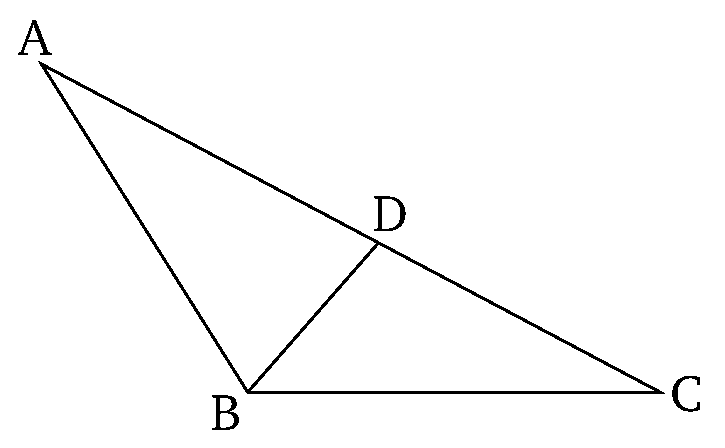
\includegraphics[width=0.5\linewidth]{figures/fig18e.eps}
    \label{fig:prop_18}
    \end{center}
\end{figure*}

In any triangle, the greater side subtends the greater angle.

For let $ABC$ be a triangle having side $AC$ greater than $AB$. I say that
angle $ABC$ is also greater than $BCA$.

For since $AC$ is greater than $AB$, let $AD$ be made equal to $AB$
 [Prop.~1.3],
and let $BD$ have been joined.

And since angle $ADB$ is external to triangle $BCD$, it is greater than the
internal and opposite (angle) $DCB$ [Prop.~1.16]. But $ADB$ (is) equal to $ABD$,
since side $AB$ is also equal to side $AD$ [Prop.~1.5]. Thus,
$ABD$ is also greater than $ACB$. Thus, $ABC$ is much greater than 
$ACB$.

Thus, in any triangle, the greater side subtends the greater angle.
(Which is) the very thing  it was required to show.


\section*{Commentary}

\begin{proposition}\label{proposition_18}\lean{Elements.Book1.proposition_18}\leanok
    In $\triangle~ABC$, if $|AC|~>~|AB|$, then $\angle~ABC~>~\angle~BCA$
\end{proposition}
\begin{proof}
    \uses{proposition_3,proposition_5',proposition_16}\leanok
    See the original proof by Euclid.
\end{proof}
